% !TeX root = ../main.tex

\clearpage
\section{Lessons from Preliminary Experiments}\label{appendix:prior-experiments}

Several approaches preceded the stereo-depth alignment method developed in
this thesis. They explored filtering codec motion, using it to propagate
existing image features, and changing the lifetime or placement of tracked
samples. The examples below come from archived development experiments on
Monado sequences~\cite{deMayoCremersPireMSD}. Some used image features, inertial
rotation, or ground-truth geometry to investigate particular limitations; they
are separate from the final pixel-free EuRoC evaluation. Their common lesson
is that useful local motion and persistent point identity are distinct
requirements.

\subsection{Frequency-Based Selection of Motion Vectors}

An early idea was to distinguish coherent camera-induced motion from irregular
codec predictions through their frequency content. Motion-vector fields were
sampled on an eight-pixel grid and decomposed into spatial or spatiotemporal
frequency bands. A complementary temporal diagnostic compared successive
fields after alignment using the coded displacements. For two aligned motion
samples $\mathbf{m}_a$ and $\mathbf{m}_b$, the normalized two-point Fourier
transform has coefficients
\begin{equation}
  \frac{\mathbf{m}_a+\mathbf{m}_b}{2}
  \quad\text{and}\quad
  \frac{\mathbf{m}_a-\mathbf{m}_b}{2}.
\end{equation}
The second coefficient measures disagreement between the samples. A small
value suggests temporal consistency, but can also occur when both samples
share an incorrect displacement. A three-dimensional FFT over the two-frame
volume additionally measures spatial variation.

The diagnostic assigned each vector to the frequency band with the largest
reconstructed magnitude, provided that band's share of the summed magnitudes
exceeded a chosen dominance threshold. Spatial and spatiotemporal bands used
normalized radial cuts of 0.12 and 0.35.

\begin{figure}[!htbp]
  \centering
  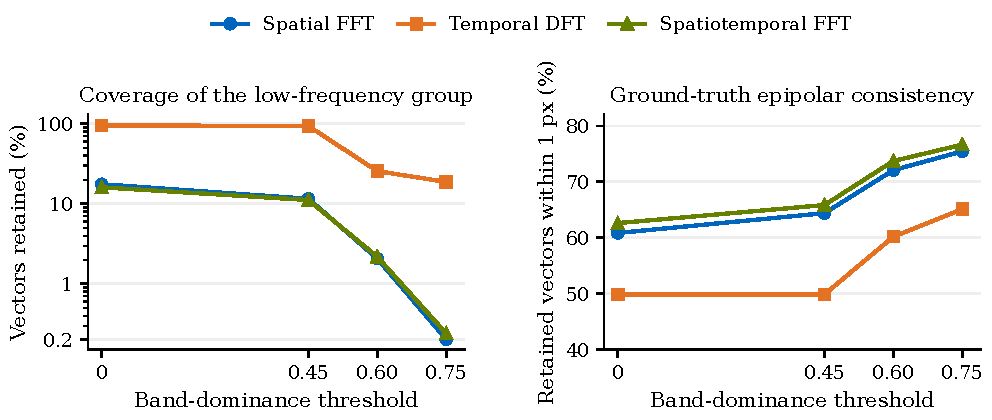
\includegraphics[width=\textwidth]{figures/appendix/prior-fft-coverage-consistency}
  \caption[Frequency selection: coverage and epipolar consistency]{Low-frequency
  selection on MOO06. Coverage uses a logarithmic axis. Consistency measures
  the fraction of retained vectors with ground-truth square-root Sampson
  residual at most one pixel, evaluated in undistorted coordinates and scaled
  by $\sqrt{f_xf_y}$. Spatial grouping covers 7,108,462 vectors; the temporally
  aligned methods cover 7,017,517 because they require a preceding field.}
  \label{fig:prior-fft-selection}
\end{figure}

\autoref{fig:prior-fft-selection} shows the resulting trade-off on MOO06.
At a threshold of 0.45, the spatiotemporal low-frequency group retained
11.15\% of the input vectors; 65.85\% of those satisfied the one-pixel
ground-truth epipolar check. Raising the threshold to 0.75 increased that
fraction to 76.65\%, but retained only 0.24\% of the vectors. Frequency
selection could therefore enrich a geometrically consistent subset at a
substantial cost in coverage. Even a small epipolar residual does not
establish the correct endpoint along the epipolar line or the identity of a
physical scene point.

A later variant ranked blocks by the sum of their reconstructed band
magnitudes and selected up to ten translation-support correspondences from
low-ranked blocks containing active features, for an inertial-rotation-assisted
epipolar filter. This score was called ``energy'' during development, although
it was not squared Fourier energy. Without image refinement of these
supports, global ranking produced \SI{0.538}{\metre} ATE RMSE on the full
4,171-frame MOO06 run, compared with
\SI{0.177}{\metre} for image-refined translation support. Selecting supports
within spatial windows improved the ranked variant to
\SI{0.299}{\metre}. These run-level results evaluate support sets, not the pose
consistency of the single lowest-scoring vector; they therefore do not settle
the latter question.

\subsection{Propagating Existing Features}

Another approach retained the identities of existing image features and
propagated their coordinates with codec displacements. At each transition,
it selected a motion vector whose source support contained the current
feature location, applied that vector, and stored the endpoint under the
same track ID. The attraction was to reuse an established feature-based
backend while replacing repeated temporal image matching. However, carrying
an ID forward does not verify that its new coordinate still observes the
same physical point.

\autoref{fig:prior-mv-propagation} illustrates the difference between a
promising short run and sustained tracking on MIO07. The archived direct-MV
prototype reached approximately \SI{0.096}{\metre} ATE over its first 800
frames, but approximately \SI{30.27}{\metre} over the full 4,095-frame
sequence. The image-based reference finished at approximately
\SI{0.120}{\metre}. The prototype still assigned vectors to 92.8\% of
attempted feature propagations. That count describes available assignments,
not their geometric correctness or preservation of point identity.

\begin{figure}[htbp]
  \centering
  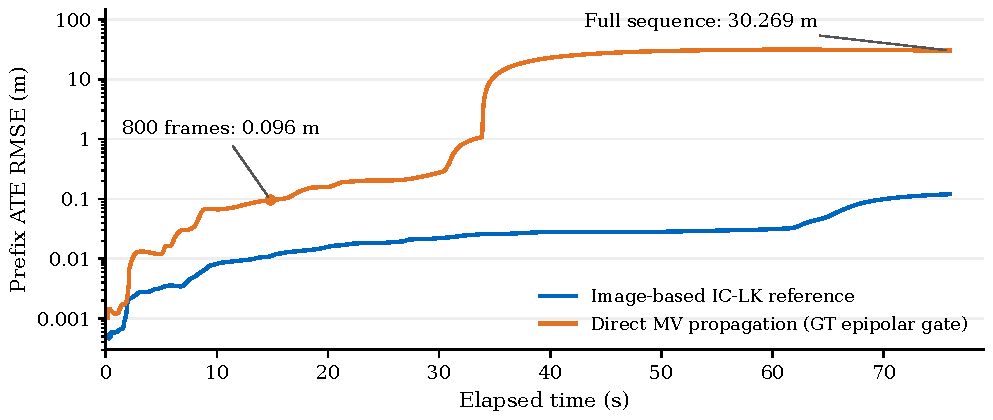
\includegraphics[width=\textwidth]{figures/appendix/prior-mv-propagation-prefix-error}
  \caption[An early direct-MV propagation failure]{Archived MIO07 development
  run: direct temporal MV propagation and an image-based inverse-compositional
  Lucas--Kanade reference. Each plotted ATE is evaluated over the prefix ending
  at that time, with a new rigid alignment and fixed scale for that prefix.
  The vertical axis is logarithmic. The direct-MV prototype used a
  ground-truth epipolar gate with a loose 32-pixel threshold, retaining
  99.6\% of input vectors; it was not an oracle for correct point identity.
  Image-based feature detection and stereo matching were retained; codec
  vectors replaced temporal tracking only.
  The curves are redrawn from the archived per-prefix measurements and do not
  represent the final PVO configuration.}
  \label{fig:prior-mv-propagation}
\end{figure}

This failure does not isolate identity drift as its sole cause: geometric
support, stereo observations, and backend conditioning also matter. It shows
why short-prefix accuracy and high assignment counts were insufficient
validation. The feature-seeded diagnostic in
\autoref{fig:mv-feature-departure-example} shows a local mechanism: codec
propagation can depart from an image track despite a common starting point
and continuing vector support.

\FloatBarrier
Further tests examined feature placement and temporal connectivity
separately. In a stereo-inertial test with spatial refill opportunities
controlled, using arbitrary codec block centres as starting locations
reduced successful temporal KLT
counts to 35.8\% of the FAST-location reference on MIO07 and 37.1\% on
MOO07. This experiment retained image-based tracking and did not use codec
displacements; it showed that block centres were not interchangeable with
selected image features. In a separate visual-only stereo test on 800 MIO07 frames using KLT
correspondences, restricting landmarks to adjacent frame pairs produced
\SI{0.521}{\metre} ATE. Making every frame a keyframe improved this to
\SI{0.035}{\metre}, while persistent tracks achieved
\SI{0.011}{\metre}. Shorter identities therefore also required changes to
landmark admission and map connectivity; they were not a complete solution
on their own.

\subsection{Persistent Surfaces with Changing Point Support}

These observations suggest a direction beyond improving a point-selection
rule. The useful codec support on an extended surface can change from frame
to frame. For example, observations on a tabletop might shift between its
edge, a corner, and an interior textured region. Such observations may remain
compatible with the motion of the same static surface even when they cannot
be joined into one long-lived point track. This is a motivation for testing
surface-level association, not evidence that the present experiments already
recover object identities.

Li and Song~\cite{li2014toward} provide a relevant precedent under a planar
scene model. They group codec correspondences using homography RANSAC,
associate planes across frames, and jointly estimate plane geometry and
camera motion in an extended Kalman filter. Their state can retain a plane
while its supporting point correspondences change. The observation model
still uses those correspondences through a plane-induced homography; the
plane label alone does not supply camera motion.

A future codec-based estimator could similarly maintain a static plane or
other geometric region while renewing its short-lived correspondence support.
It would need reliable region association, enough spatially distributed
observations, and geometry that constrains the camera motion. Merely seeing
another part of the same object would not satisfy these requirements.
Non-planar objects would require an appropriate shape or rigid-body model,
and independently moving objects would need separate treatment. Preserving
the pixel-free boundary would also require forming and associating these
regions from codec metadata and geometry. The stereo-depth construction in
this thesis supplies one possible source of that geometry; whether a surface
representation makes better use of intermittent codec support remains an
open experimental question.
